\def\chapdir{./ChapterIntro}

\chapter{Introduction} \label{ch:intro}

\section{Project Overview}

OllamaNet is a comprehensive AI platform built on a modern microservices architecture that enables its users to explore, interact with, and manage various AI models through a coherent ecosystem of services. The platform provides both administrative capabilities and end-user experiences for AI-powered conversations and model discovery, all supported by a robust database layer.

The platform is designed to address the growing need for accessible, well-organized AI model interactions while maintaining security, scalability, and performance through specialized microservices that handle distinct aspects of the system's functionality.

A key purpose of OllamaNet is to provide developers with a customizable and scalable infrastructure for working with Large Language Models (LLMs), offering an alternative to existing Python-based libraries that may lack performance and customization options. By leveraging C\# and .NET, the platform delivers superior robustness, maintainability, and extensibility, opening pathways for custom extensions and enterprise-grade implementations.

\begin{figure}
    \centering
    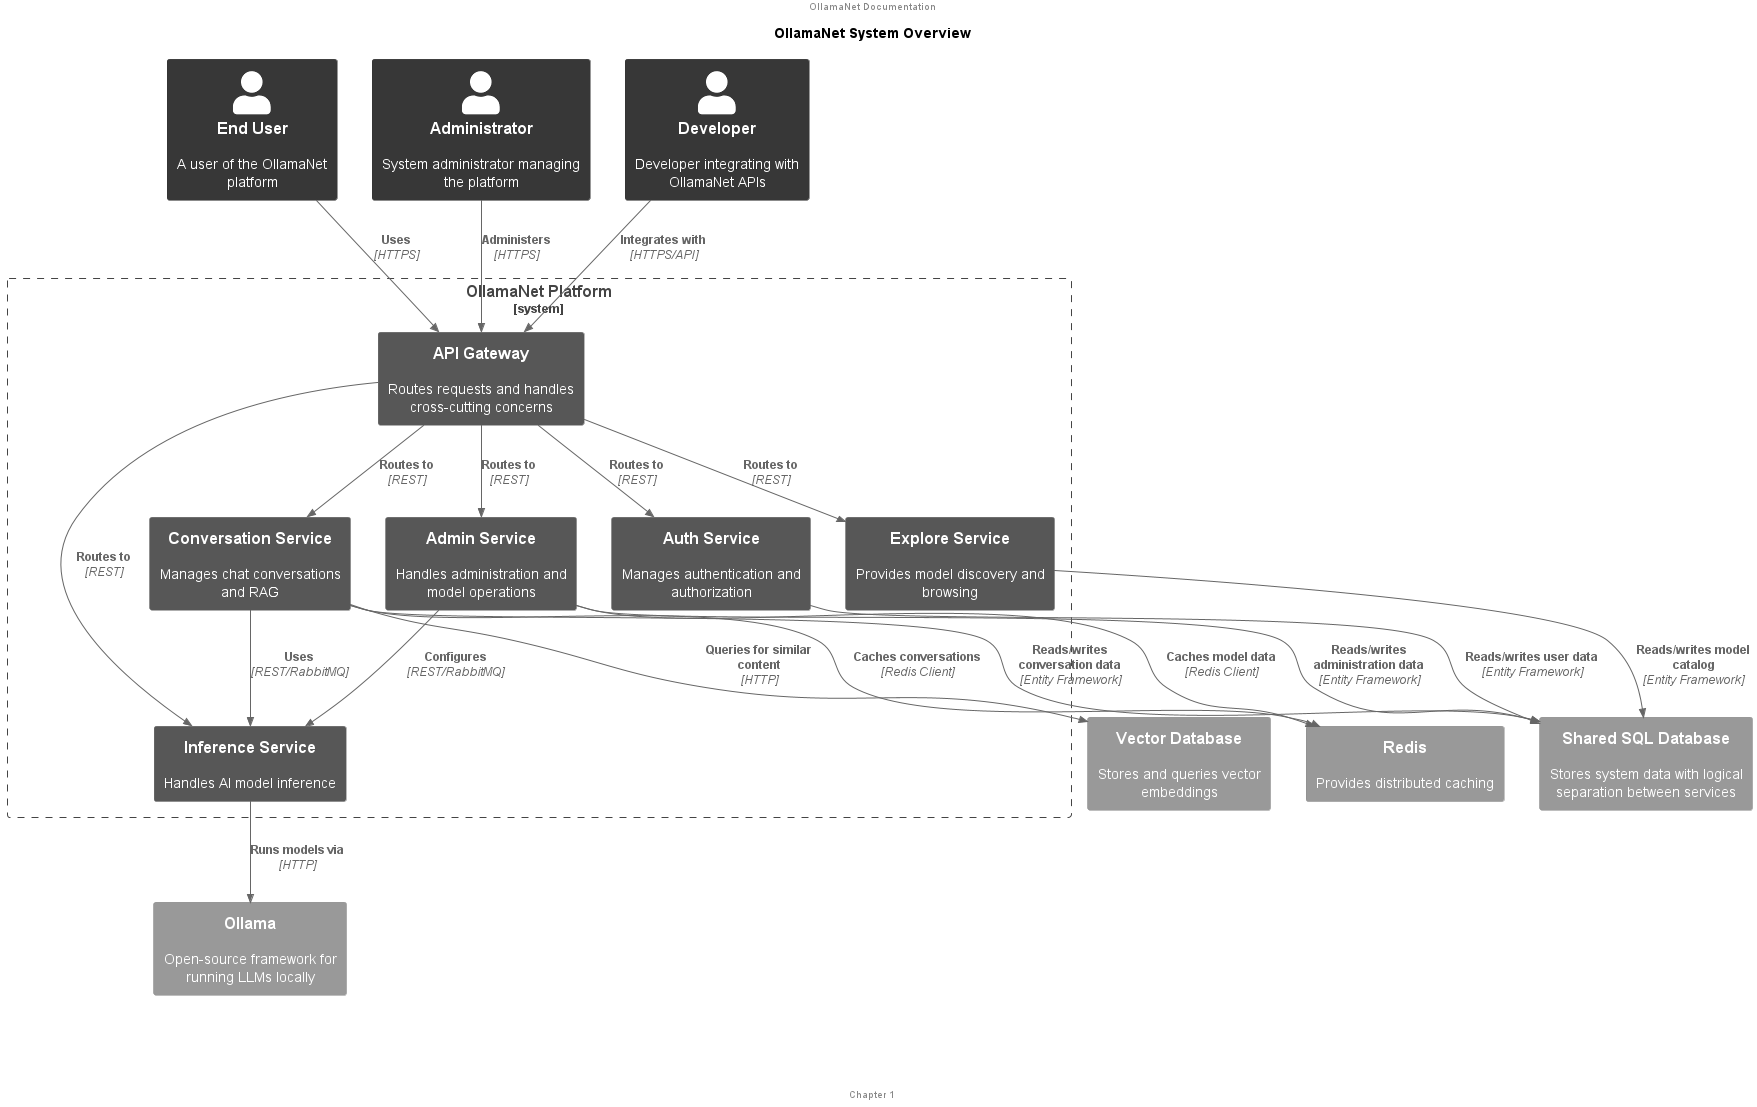
\includegraphics[width=0.8\textwidth]{./Chapter01/figures/OllamaNet_System_Overview.png}
    \caption{OllamaNet Architecture Overview}
    \label{fig:ollamanet-architecture}
\end{figure}

\begin{terminology}
\begin{description}
    \item[OllamaNet:] Comprehensive AI platform with microservices architecture for LLM interaction
    \item[Microservice:] Independent, specialized service with specific domain responsibilities
    \item[LLM:] Large Language Model, an AI model used for text generation and understanding
\end{description}
\end{terminology}

\section{Problem Statement}

Traditional AI model deployment and interaction platforms often face several key challenges:

\begin{enumerate}
    \item \textbf{Complexity in Administration}: Managing AI models, users, and permissions typically requires complex administrative interfaces.
    \item \textbf{Context Loss in Conversations}: Users often lose conversation history and context when interacting with AI models.
    \item \textbf{Inefficient Discovery}: Finding the right AI model for specific needs can be difficult without proper categorization and search capabilities.
    \item \textbf{Security Concerns}: Maintaining proper authentication and authorization across AI services presents security challenges.
    \item \textbf{Performance Bottlenecks}: AI interactions can suffer from latency issues, especially without proper caching and optimization strategies.
    \item \textbf{Data Management Complexity}: Handling the persistence of conversations, user data, and model information requires sophisticated data access patterns.
    \item \textbf{Reliability Constraints}: Many existing solutions use non-relational databases for speed of development, sacrificing data reliability and relationship integrity in the process.
    \item \textbf{Limited Customization}: Popular Python-based LLM libraries prioritize simplicity over extensibility, limiting developers' ability to customize the infrastructure.
\end{enumerate}

OllamaNet addresses these challenges through its specialized microservice architecture, providing a robust, extensible, and maintainable solution for AI model interaction.

\begin{terminology}
\begin{description}
    \item[API Gateway:] Component that routes requests to appropriate microservices
    \item[Context Preservation:] Maintaining conversation history and state across interactions
    \item[Caching:] Storing frequently accessed data to improve performance
\end{description}
\end{terminology}

\section{Objectives and Goals}

The OllamaNet platform aims to achieve the following objectives:

\begin{enumerate}
    \item \textbf{Provide Comprehensive Administration}: Deliver complete control over platform resources through the AdminService.
    \item \textbf{Enable Secure Authentication}: Implement robust user authentication and authorization via the AuthService.
    \item \textbf{Facilitate Model Discovery}: Allow users to browse and evaluate AI models through the ExploreService.
    \item \textbf{Support Rich Conversations}: Enable persistent, organized conversations with AI models via the ConversationService.
    \item \textbf{Ensure Data Integrity}: Maintain consistent data operations through the DB Layer.
    \item \textbf{Optimize Performance}: Implement caching strategies and efficient data access patterns across services.
    \item \textbf{Enhance User Experience}: Deliver a responsive, intuitive interface for all platform interactions.
    \item \textbf{Enable Custom Inference}: Provide flexible AI model inference capabilities through the InferenceService.
\end{enumerate}

These objectives are achieved through a carefully designed microservices architecture that emphasizes separation of concerns, domain-driven design, and robust integration patterns.

\begin{terminology}
\begin{description}
    \item[Domain-Driven Design:] Software development approach that focuses on the core domain and domain logic
    \item[Separation of Concerns:] Design principle for separating software into distinct sections
    \item[Integration Pattern:] Standardized approach for connecting different components or services
\end{description}
\end{terminology}

\section{Project Scope}

OllamaNet encompasses a full-stack solution with the following components:

\subsection{Microservices Backend}
\begin{itemize}
    \item \textbf{AdminService}: Central control point for platform administration, managing users, AI models, tags, and inference operations.
    \item \textbf{AuthService}: Comprehensive authentication and authorization service handling user registration, login, password management, and role-based access control.
    \item \textbf{ExploreService}: Model discovery and browsing service allowing users to search, filter, and explore available AI models and their capabilities.
    \item \textbf{ConversationService}: Conversation management service enabling persistent, organized interactions with AI models, including real-time streaming responses.
    \item \textbf{InferenceService}: Flexible inference engine service for interacting with Ollama models, exposed via ngrok for accessibility.
    \item \textbf{Gateway}: API gateway service routing client requests to appropriate microservices, handling authentication and authorization.
    \item \textbf{DB Layer}: Shared data access infrastructure implementing the repository and unit of work patterns for consistent data operations.
\end{itemize}

\subsection{Frontend Applications}
\begin{itemize}
    \item Administrative interfaces for platform management
    \item End-user interfaces for conversation and model exploration
\end{itemize}

\subsection{Infrastructure Components}
\begin{itemize}
    \item SQL Server database for persistence
    \item Redis for distributed caching
    \item JWT-based authentication system
    \item Integration with the Ollama inference engine
    \item RabbitMQ for service discovery
\end{itemize}

\begin{figure}
    \centering
    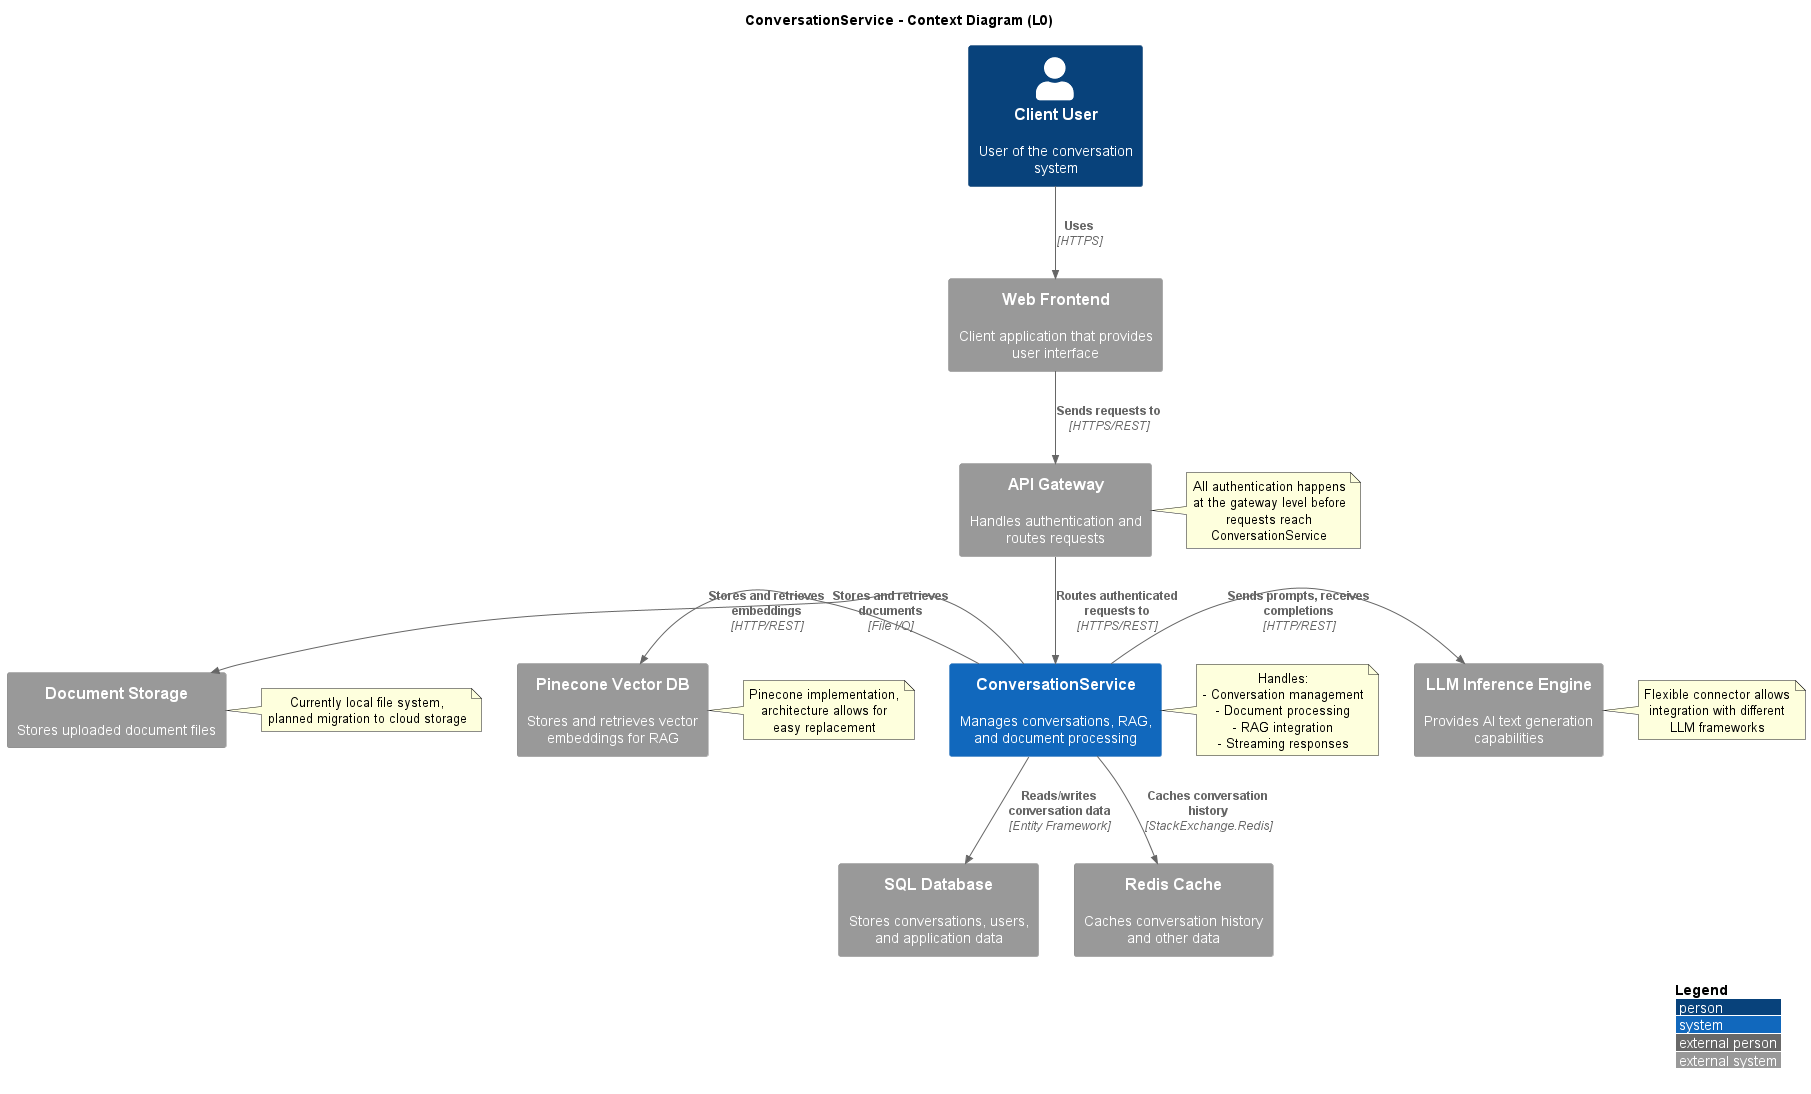
\includegraphics[width=0.8\textwidth]{./Chapter01/figures/ConversationService_Context.png}
    \caption{OllamaNet Platform Components}
    \label{fig:ollamanet-platform-components}
\end{figure}

\begin{terminology}
\begin{description}
    \item[Repository Pattern:] Design pattern that mediates between the domain and data mapping layers
    \item[Unit of Work:] Pattern that maintains a list of objects affected by a business transaction
    \item[JWT:] JSON Web Token, a secure method for representing claims between parties
    \item[Redis:] In-memory data structure store used for caching
    \item[RabbitMQ:] Message broker software for service-to-service communication
\end{description}
\end{terminology}

\section{Implementation Strategy}

OllamaNet follows a structured implementation approach:

\begin{enumerate}
    \item \textbf{Service Isolation}: Each microservice addresses a specific domain with clear boundaries, following domain-driven design principles.
    \item \textbf{Shared Data Layer}: A common DB layer provides consistent data access patterns across all services.
    \item \textbf{API-First Design}: RESTful APIs with comprehensive documentation via Swagger/OpenAPI ensure clear service interfaces.
    \item \textbf{Progressive Enhancement}: Services evolve through phased migrations and improvements, with clear versioning.
    \item \textbf{Performance Optimization}: Strategic caching and efficient data access patterns ensure responsive user experiences.
    \item \textbf{Security Integration}: Consistent authentication and authorization across services protect resources.
    \item \textbf{Domain-Driven Design}: Service organization based on business domains and use cases ensures alignment with business needs.
    \item \textbf{Notebook-First Inference}: The InferenceService uses a notebook-based architecture for flexibility and accessibility.
\end{enumerate}

This implementation strategy enables the platform to be both robust and flexible, catering to enterprise-grade requirements while maintaining developer accessibility and extensibility.

\begin{terminology}
\begin{description}
    \item[REST:] Representational State Transfer, an architectural style for designing networked applications
    \item[Swagger/OpenAPI:] Framework for API documentation and specification
    \item[Notebook-First Architecture:] Implementation approach that prioritizes interactive development environments
\end{description}
\end{terminology}

\section{Report Structure}

This documentation is organized to provide a comprehensive understanding of the OllamaNet platform:

\begin{itemize}
    \item \textbf{Chapter 2}: Explores the background and theoretical foundations of microservices architecture
    \item \textbf{Chapter 3}: Details the requirements analysis and domain modeling
    \item \textbf{Chapter 4}: Describes the overall system architecture and communication patterns
    \item \textbf{Chapter 5}: Examines the database layer and data management strategies
    \item \textbf{Chapter 6}: Provides detailed designs for each microservice
    \item \textbf{Chapter 7}: Outlines the frontend architecture and integration
    \item \textbf{Chapter 8}: Explains the testing strategy across services
    \item \textbf{Chapter 9}: Covers implementation details and development practices
    \item \textbf{Chapter 10}: Presents system evaluation and performance metrics
    \item \textbf{Chapter 11}: Concludes with lessons learned and future directions
\end{itemize}

Each chapter builds on the previous to create a complete picture of the OllamaNet platform's architecture, implementation, and value proposition.

\begin{terminology}
\begin{description}
    \item[Architecture:] The high-level structure of a software system
    \item[Domain Model:] Conceptual model of the domain that incorporates both behavior and data
    \item[Communication Pattern:] Standard approach for service interactions in a distributed system
\end{description}
\end{terminology}





